\section{Spacky follows a crowd}
\begin{multicols}{2}
\subsection{A view from a hilltop}
  \begin{aloud}
  A mid-spring sunset is shining down on your back.
  You are past the eastern border of the Thornic Empire, in the sprawling grasslands
    nicknamed the Wastes.
  You and the rest of your band, the Crazy Kua-Toa, have been tracking a Gnoll warband for the
    better part of a week, making sure you will be able to warn the nearby bordertown,
    Celadir's Bastion, if it looks like they plan to attack.
  \end{aloud}

You've pitched camp not far from the treacherous edge of the Merlicut Gorge.
The gorge carves an impossibly straight line that defines the eastern edge of the Empire,
  a quarter-mile wide and hundreds of feet deep, with a strong river at the bottom that runs
  the short distance remaining to the southern seas.
Your band often camps near the gorge, partially for the safety of a natural defense, and partially
  to make it easier to find camp -- walk to the gorge, and then you've got a 50/50 chance
  picking the right direction towards camp.

A small fire burns in a low-dug fire-pit, the hardwood abundant here thankfully giving off
  almost no smoke.

The mountain dwarf Gluri Frosthand, the band's leader, chews one some dried meat while watching
  the fire contemplatively.
He scratches at the perpetual sunburn on his bald head with the three fingers of his ruined right
  hand.
An uglier man you've never met, and as much as he loves his goatee, it really isn't helping.
But he's a compotent leader, respectful, and fair.

The middle-aged human Garr Bolbec, your band's runner, is reclined and smoking, absentmindedly
  blowing gouts of smoke through the braids of his enormous beard.

The high elf Lilith, the band's muscle, patrols to the east of your camp, walking north and south
  and back, well outside the circle of the fire to preserve her night vision.
She is one of the most talented people you've ever seen with a blade and perhaps the most
  terrifying woman you've ever met.
She looks like a fine painting salvaged from a castle under siege.
Her proud bearing, high cheekbones, and piercing eyes give her a regal air, but a puckered scar
  runs from the missing tip of her nose, under her right eye, down to the corner of her lips,
  and around her jaw.

Lastly, Ogden, the band's frontman, is afield, maintaining a bead on your quarry.
The warband has stopped for the time being, but you'll need to know quickly if they beging to move
  again.
Ogden looks like a fairytale prince had a bad run through the gladiator pit.
[Just read the block?]


\hrulefill

The next day, shortly before sunrise, the five of you are return to a nearby hill from which you
  can see the edge of the warband.
Per an unspoken standard, Ogden and Lilith hold back and keep watch for trouble from the rear,
  Gluri and you proceeding to the peak of the hill.

Off and on for the last week, the warband would either sit still for a day, or move north.
You're waiting to see which it will be.

[If they didn't talk over the fire, Gluri will mention that he doesn't like how straight-line
 the gnoll have been moving.]

Maybe chat.

ou expect the warband to continue on its way north, but it doesn't move.
Instead, a small group of half a dozen gnoll break off from the main body.

Pick Nature or Arcana

Nature 15: You know that gnolls are generally nomadic, moving as an entire group.
Historically, they would raze villages, but ever since Shomah and the Defiant founded the Empire
  and pushed most of the beast races into the Wastes, they've had to settle for razing other
  camps of beastmen.
There are rumors of settlements farther to the east, which could conceivably offer a target to the gnoll.
But either way, detachments aren't a thing gnolls really do.
Suffice it to say, this is wieeeeeeeerd.


The gnoll at the front of the group wears half a still-rotting skull.
Just behind that one, a great brute of a gnoll.
Four runts trail behind those two.

Roll Religion 15:
  You know that gnoll were created by and worship the demon-god Yeenoghu, the Beast of Butchery.
  The gnoll at the front is a Fang of Yennoghu.
  By dark power bestowed by their demon-god, a Fang can turn hyena and wolves into gnolls.
  While not abundant in the hostile Wildes, the presence of this Fang represents an upcoming
    boom in the gnoll population.


  The dwarf holds a spyglass in his left hand while nervously tugging on his medium-length goatee
    with the three remaining fingers of his ruined right hand.
  You are watching the immediate area while he spys on whatever it is he sees.
  Gluri emits a sound halfway between a grunt and a growl.
  \end{aloud}

Converse.
Hand Spacky the looking glass.
``What do you make of this shit?''

Roll Perception?
On a bad roll, Gluri has to assist and call out where it is.

  \begin{aloud}
  You see a hundred or more Gnoll milling around.
  Half a dozen Gnoll have separated from the main host, heading north.
  Following along their heading, you see they are jogging out to meet a woman standing alone
    in the tall grass.
  She has sickly, greenish skin, nappy black hair, and is wearing a tattered red evening gown.
  She moves listlessly, running her hands low through the grass.
  \end{aloud}

15 to notice the grass bend in a way that suggests there are things moving through it.
Oppose a +4 Stealth to see a glint of scales.

DC 20 Nature to identify the Yuan-ti.
Advantage if previous DC 15 was successful.

Converse.
``It's not fucking good, I'd bet that.
[Pause a beat.]
We better head back.
Garr'll need to run a message.''

A gnoll scout is returning from the west, over the hill you are on.
Perception and Stealth (+1).
\end{multicols}

\pagebreak
\subsection{Combat}
For Gluri, use Duergar base stats and weapons attacks (no resistance or magic).
\begin{multicols}{2}

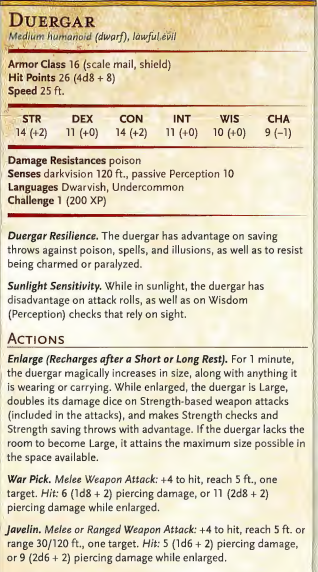
\includegraphics[width=\linewidth,keepaspectration=true]{img/statblock/duergar-clipped.png}

\columnbreak

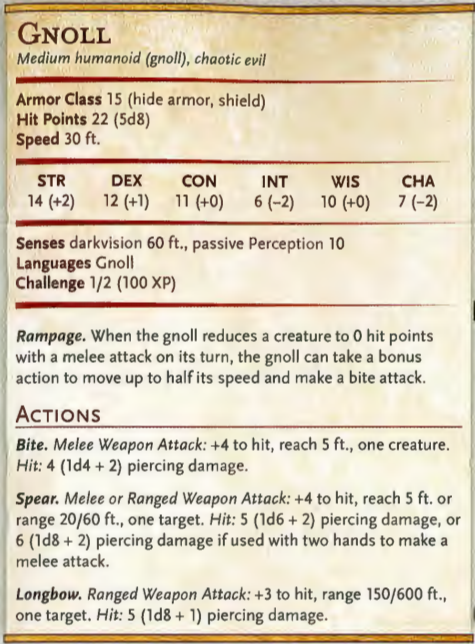
\includegraphics[width=\linewidth,keepaspectratio]{img/statblock/gnoll.png}

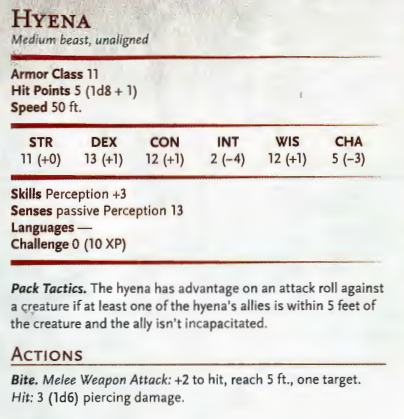
\includegraphics[width=\linewidth,keepaspectratio]{img/statblock/hyena.png}
\end{multicols}

\pagebreak

\begin{multicols}{2}
\subsection{Return to camp}
``Collect the thumbs.''

Your trek back to camp is uneventful.
You head west until you get to the Gash, the graet, wide, and long canyon that separates the
  Wastes from the Empire.
You always make your camp somewhere along its edge, half so you can always trust that you can find
  it, and half because the beastmen rarely come close to it.
You eventually find your campsite.

  \begin{aloud}
  You hear them before you see them.
  Ogden, the band's frontman, and Alotel, the band's muscle, are arguing in the hissing, short
    tones of two people barely keeping themselves from yelling.
  Nearer, Garr, the band's message runner and half-assed minstrel, is reclining against a stump,
    alternating between tending a decently sized fire and idly strumming a lute.
  Nearby, a large, multi-legged, and recently beheaded lizard is hung from a tree branch,
    blood draining down a shallow, fresh ditch that runs west, into the Gash's canyon.
  \end{aloud}

  [Pause a beat in case Spacky comments.]
  Gluri asks ``What's crawled up their asses?''
  Garr responds in his heavy accent.
  ``I stay out it.''

  \hyperref[description:ogden]{[Describe Ogden]}.

  \hyperref[description:alotel]{[Describe Alotel]}.

  ``I see your hand twitching for your knives, child.
    I'll show you a terrible way to die, if that's what you're after.''

  Ogden is seething.
  He shoves a finger in Alotel's face.
  He is almost sad when he says,
  ``You don't know what you're talking about, you ignorant cunt.''

  Pause a beat, see what Spacky wants to do.
  Let him defuse the situation if he can.

  A few heartbeats pass before Gluri clears his throat and speaks calmly, conversationally.
  ``What \emph{is} she talking about, Ogden?''
  The two bruisers startle to see you there, turning quickly to abashed, like children caught
    misbehaving.
  Which, in a way, given Gluri's leadership, they are.
  Gluri continues in his calm, low rumble.
  ``What's got you so riled up that you're making enough noise that the Horde could hear you?
    And tell me, why the fuck is no one keeping watch for whatever you two hissing alleycats are
      about to bring down on us, eh?''
  If Spacky doesn't calm tensions, Gluri pulls rank and demands them separate.

  After everyone is either calm or gone elsewhere, Gluri says
  ``I saw something back there that looked like it could almost be edible.
    See it gets cooking, eh?''

  Garr has set up everything you need: a roasting spit, a banked fire full of hot coals.
  He's even set out some good knives for you to field dress the beast,
    filled a bucket with water, and pulled the beast down off the branch, now that it's mostly
    dripped dry.

  If prompted to dress the animal himself: ``I do not cut.  You know this.''
  While it's never been a conversation with Garr, you realize that no, you've never seen him hold
    so much as a knife, never mind a sword or other weapon.

  Roll some Surivial checks, just for sport.
  On bad rolls, maybe it takes a long time to get everything squared away.
  Set to roasting this thing.
  You know it's going to take a few hours of steadily turning it, but it's a pleasant day out
    and the work is done.
  People come and go, rotating on and off sentry duty.

\subsection{Ghost stories}

  It's later.
  The roasting beast has started smelling pretty good.
  Wind is blowing from the east, so you don't think it'll attract any of the beastmen tonight.

  The band is seated around the fire.
  Garr is somewhat removed with his back to the fire, keeping a lazy watch while not ruining his
    night vision.
  The group chatters about nothing in particular.
  Lulls of cold silence are frequent, if Specky allows them.

  If not otherwise directed, Gluri will prompt
  ``Alright, we can't keep any bad blood between us.
    What is it you two were arguing about earlier?''
  Alotel will just scowl.

  Ogden will start with
  ``Look, we've all got our shit, right?
    Nobody not crazy joins a band.
    Can we just leave it at that?''

  Ogden will sigh and say,
  ``I killed a basilisk today.
    The head'll get a bounty, sure, and its eye'll fetch a price from the wizard, fine.
    But that's not why I hunted it down and killed it.
    I did it because, no matter what that woman says, a basilisk is one of the most terrible
      fucking abominations in the whole of creation.''

  [Beat.]  Gluri, ``That's it?  That was your big argument?''
  Alotel snorts, throws her hands up in an \emph{I know, right?} expression.
  Ogden draws a breath to retort, but stops himself.
  He grins, saying
  ``You know what?
    Fine.
    Let's make a game of it, then.
    Let's talk about our fucking feelings.
    [Beat.]
    You tell me the worst piece of agony you've been made to endure?
    You all tell me that, and I'll tell you why a basilisk makes it look like a day-long free pass
      to your favorite whorehouse.
    [Beat.]
    No?
    You don't feel like talking all of a sudden?''


  Again, see if Spacky will take the lead.
  Otherwise, in no particular order.

  \hline

  Gluri has mentioned before that his childhood home was raided and ruined by the Duergar.
  He never mentioned before that he lived there for almost a century.
  Old enough to be a man.
  Old enough to have a wife.
  To have a whelp.

  \hline

Garr doesn't turn around.
  He holds up his left hand, exposing the brand that he has, before now, always refused to explain.
  ``Before now, all it.
    Then, I am animal.''
    He motions vaguely eastward.
  ``Like the dog men.
    Master tell fight, I fight.
    Tell kill, I kill.
    I am dog for master.

    This all bad, is not most bad.
    Most bad is think.
    Many times, I not fight master.
    Many times, I am dog and not man.
    Much hurt, afraid of master hurt me.

    When kill master, no [pause]'' search for the word ``joy.
    I think kill make joy, make man.
    Only make know, would better do long before.''

  \hline

  Alotel stares at the fire.
  ``I was in a house on fire.
    Never mind the smoke, you can't breathe for the heat of it.

    I was\dots trapped.
    The fire spread into my room.
    I could feel my skin bubble.
    The pain.
    [snort]
    The smell.
    I'll never forget it.

    [shake head, break from reverie]
    The ropes caught fire.
    I got out.
    Even limping, I caught up with them on the road a few days later.
    My whole body cooked, weeping puss.

    Killed them in their sleep with their own knives.
    And Garr's right.
    It wasn't satisfying.''

  \hline

  ``They're not hard to kill.
    They're slow and lumbering.
    But it's the risk.
    They can turn you to stone if you're careless, and that's the worst fucking way in the world
      to go.''

  [pause]
  Spent three hours petrified.
  Worst day of my life.

  how'd you get out

  One of the stomachs has an acid in it.
  Mix it with lemongrass and slather it everywhere.
  It only works if you've only been stone for a little bit.
  I don't pretend to understand it, but my Goldie told me that's what she did, and I've never had
    reason to doubt her.


\end{multicols}

